\documentclass{article}
\title{Blanchard Ch.17}
\author{Dawei Wang}
\date{\today}
\usepackage{ctex}
\usepackage{amsmath}
\usepackage{amssymb}
\usepackage{graphicx} %插入图片的宏包
\usepackage{float} %设置图片浮动位置的宏包
\usepackage{subfigure} %插入多图时用子图显示的宏包
\begin{document}
	\maketitle
开放有三个不同的方面:

产品市场开放(openness in goods markets)——消费者和公司在本国市场和外国市场之间进行选择的能力。没有任何一个国家对这种自由是毫无限制的,即使是贸易程度最高的国家至少也会对一些外国产品实行关税(tariff)和配额(quotas)。

金融市场的开放(openness in financial markets)——金融投资者有在本国资产和外国资产之间进行选择的能力。即使是世界上最富有的国家仍然有资本管制(capital controls),即对本国居民持有外国资产的数量以及外国人持有本国资产数量的限制。

要素市场的开放(openness in factor markets)——公司选择生产地点和工人选择工作地点的能力。

相比于产品市场或者金融市场的开放,要素市场开放的作用较小。因此忽略要素市场的开放。

\section{产品市场的开放}

贸易余额:出口和进口的差额:如果出口超过进口,就存在贸易盈余;如果进口超过出口,就存在贸易赤字。

考虑到出口和进口可能包括中间产品的进口和出口,而GDP是指经济中的增加值。因此出口可以超过GDP。

\subsection{本国产品和外国产品间的选择}

是购买本国产品还是外国产品的决策,核心在于本国产品相对于外国产品的价格。我们称这个相对价格为实际汇率(real exchange rate)。

在一个封闭经济中,人们面临的决策是购买还是储蓄;在一个开放经济中,人们面临两个决策:储蓄还是购买,购买本国产品还是购买外国产品。

\subsection{名义汇率}

名义汇率的两种表现形式:

用外国货币形式表示的本国货币价格。

用本国货币形式表示的外国货币价格。

\hspace*{\fill}

采用第一种定义,此时名义利率被定义为以外币标价的本币价格,并用E表示。

本币的升值(appreciation)是指用外币标价的本币价格的提高。给定我们对汇率的定义,本币的升值对应着汇率E的上升。

本币的贬值(depreciation)是指用外币标价的本币价格的下降。因此本币的贬值对应着汇率E的下降。

\hspace*{\fill}

在固定汇率国家中,汇率的上升是就是高估(revaluations),汇率下降被称作低估(devaluations)。

\subsection{从名义汇率到实际汇率}

令P表示美国的GDP平减指数,$ P^* $表示英国的GDP平减指数,E是美元-英镑的名义汇率。

\begin{figure}[H] %H为当前位置,!htb为忽略美学标准,htbp为浮动图形
	\centering %图片居中
	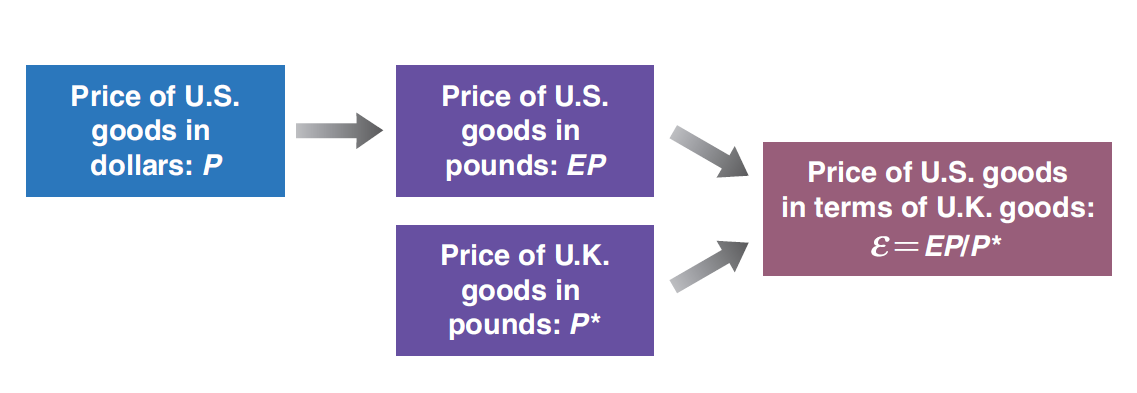
\includegraphics[width=1\textwidth]{17_1} %插入图片,[]中设置图片大小,{}中是图片文件名
	\caption{The Construction of the
		Real Exchange Rate} %最终文档中希望显示的图片标题
	\label{Fig.main2} %用于文内引用的标签
\end{figure}

美国产品的美元价格是P,乘以汇率E,即以英镑标价的美元价格,给出了美国产品的英镑价格EP。

英国产品的英镑价格为$ P^* $,实际汇率即以英国产品表示的美国产品价格,用$ \epsilon $来表示,可以由下式给出:

\[
\epsilon=\frac{EP}{P^*}
\]

$ \epsilon $:实际汇率——用外国产品表示的国内产品价格。实际汇率只是一个指数,其水平是可变的,因此不提供任何信息。尽管实际汇率水平没有什么信息,但实际汇率的相对变化却是有意义的。

\hspace*{\fill}

实际汇率上升:用外国产品表示的本国产品的相对价格提高,被称为实际升值(real appreciation);

实际汇率下降:用外国产品表示的本国产品的相对价格下降,被称为实际贬值(real depreaciation)。

名义汇率和实际汇率可以反向变动。

\[
\epsilon=E\frac{{P}}{P^*}
\]

如果E上升的同时,$ \frac{P}{P^*} $的下降程度更大,则$ \epsilon $下降。

\subsection{从双边汇率到多边汇率}

以每个国家与本国贸易往来的规模以及如何在其他国家的市场上与本国竞争为权数给每个国家赋权重,以这种方法构建的变量称之为某国多边实际汇率,或者简称某国实际汇率。(某国贸易加权实际汇率、某国有效实际汇率)。

与双边实际汇率一样,它的多边实际汇率的水平值是可变的。

\section{金融市场的开放}

金融市场的开放使金融投资者可以同时持有本国资产和外国资产,从而可以多样化其资产组合,可以对外国利率相对于本国利率的变动或汇率的变动进行投机活动。

外汇(foreign exchange),外国货币。

对一个国家而言,金融市场开放有着另外一层重要的意义。它允许一国可以有贸易盈余或者贸易赤字。如果一个贸易赤字国家从其他国家的购买要比向其他国家的出售多,那么这个国家必须向其他国家借款。他的借债是要通过吸引外国金融投资者增加他们持有的本国资产数量,实质上就是外国投资人把资金借给了这个国家。


\subsection{国际收支平衡表}

国际收支平衡表(balance of payments)

\hspace*{\fill}

经常账户(current account)

商品和服务的进出口(出口-进口=贸易余额);

本国居民从其持有的外国资产中获得收入,外国居民从其持有的本国资产中获得收入;

一个国家提供或获得外国援助(净转移支付收入,net transfers received)。

把所有向世界上其他国家支付和获得的收益加总称为经常账户余额(current account balance)。该值为正则称之为经常账户盈余(current account surplus),该值为负则称之为经常账户赤字(current account deficit)。

\hspace*{\fill}

资本账户


净外国债务:外国持有的本国资产增量减去本国持有的外国资产的增量,也叫作向本国的净资本流动(net capital flow)。

净资本流动也叫做资本账户余额(financial account balance):正的净资本流动被称为资本账户盈余(financial account surplus),负的净资本流动被称为资本账户赤字(financial account deficit)。

经常账户赤字理论上应该等于资本账户盈余,但实践中统计数据会产生统计误差(statistical discrepancy)。


国民生产总值(GNP)

GDP衡量的是本国国内的经济增加值,GNP衡量的是本国国内生产要素所带来的增加值。当经济封闭时,这两种衡量方法相同。但是,当经济开放时,它们之间就会存在差异。

国内生产要素带来的部分收入会流到国外;国内居民也可能收到部分国外收入。为了从GDP推导出GNP,我们需要从GDP开始,加上来自世界上其他国家的收入,再减去向世界上其他国家支付的收入。

GNP等于GDP加上从世界上其他国家取得的净投资收入:

\[
GNP=GDP+NI
\]

\subsection{本国资产和外国资产之间的选择}

金融市场的开放预示着人们将面临一个的新的金融决策:是持有本国资产还是持有外国资产。

这实际上涉及两个决策:是选择持有本币还是外币;是选择持有本国生息资产还是外国生息资产。人们持有货币的目的是进行交易,在本国持有外币是不能进行交易的。如果目的是持有外国资产,那么持有外币相对于持有外国债券很明显没有可取之处。因此实际只有一个需要考虑的选择:是选择本国生息资产还是外国生息资产。

(在非法活动中,外国人经常持有美元,因为美元可以容易地兑换,并且不会被追踪。在通货膨胀率极高的时期,外国人有时会换成使用外国货币,通常是美元。)

我们来考虑这些资产是一年期的本国债券和一年期的外国债券。

无拋补利率平价关系(uncovered interest parity relation),或简称利率平价条件(interest parity condition)。

\[
(1+i_t)=(E_t)(1+i^*_t)\frac{1}{E^e_{t+1}}
\]

拋补利率平价条件:

购买和持有一年期美国债券,或者在今日买进英镑,用这些英镑购买一年期的英国债券,并同意一年后以被称为远期汇率的预先价格将英镑再换回美元。这两种选择在当前都可以无风险地实现,因而它们的收益率必须相同。拋补的利率平价条件就是无风险的套利条件,它通常严格成立。

\hspace*{\fill}

这里假设金融投资者只持有最高预期收益率的债券是个很强的假设,有以下两个原因:

它忽略了交易成本;

它忽略了风险。(持有哪种债券的风险高对不同人不同,本国人持有外国债券的风险比持有本国债券的风险高)。

\subsection{利率与汇率}

\[
(1+i_t)=\frac{(1+i^*_t)}{1+(E^e_{t+1}-E_t)/E_t}
\]

近似:

\[
i\approx i^*_t-\frac{E^e_{t+1}-E_t}{E_t}
\]


投资者的套利行为预示着国内利率必然等于国外利率减去本币的预期升值率(本币的预期升值率也就是外币的预期贬值率)。


上式表明,除非有国家愿意忍受期汇率的剧烈波动,否则国内外利率很可能呈现同步变动。

\section{结论与展望}

产品市场的开放使人们可以在本国产品和外国产品之间进行选择。这个选择主要依赖于实际汇率。

金融市场的开放使人们可以在本国资产和外国资产之间进行选择。这个选择主要依赖于它们的相对收益率,而相对收益率依赖于本国和外国的利率,以及本币的预期升值率。



















\end{document}